% A complete small report: sections, maths, a table, a figure, cross-references, a bibliography and links.
% Build: pdflatex main, bibtex main, pdflatex main, pdflatex main
\documentclass[11pt,a4paper]{article}

% Packages. hyperref goes last among these, because it changes how others work.
\usepackage[T1]{fontenc}
\usepackage[margin=2.5cm]{geometry}
\usepackage{amsmath}
\usepackage{booktabs}
\usepackage{graphicx}
\usepackage{pgfplots}
\usepackage[round]{natbib}
\usepackage{xcolor}
\usepackage[colorlinks=true,linkcolor=teal,citecolor=teal,urlcolor=teal]{hyperref}
\pgfplotsset{compat=1.17}

% Your own command: change the look of every "term" from this one line.
\newcommand{\term}[1]{\textbf{#1}}

\title{Heat Loss Through a Wall}
\author{A Student}
\date{\today}

\begin{document}
\maketitle
\tableofcontents

\section{Introduction}\label{sec:intro}
A \term{U-value} measures heat flow through one square metre of a surface for each degree of
temperature difference \citep{clarke2001}. Section~\ref{sec:method} gives the equation, and
Table~\ref{tab:walls} and Figure~\ref{fig:loss} apply it.

\section{Method}\label{sec:method}
Heat loss $Q$ follows from the U-value $U$, the area $A$ and the temperature difference $\Delta T$:
\begin{equation}
  Q = U A \, \Delta T.
  \label{eq:loss}
\end{equation}
Equation~\eqref{eq:loss} is a steady-state estimate. Longer derivations line up at the equals sign:
\begin{align}
  Q &= 2.1 \times 10 \times 15 \\
    &= 315 \text{ W}.
\end{align}

\section{Results}\label{sec:results}
\begin{table}[ht]
  \centering
  \caption{Heat loss through a 10 m$^2$ wall at a difference of 15 K.}
  \label{tab:walls}
  \begin{tabular}{lrr}
    \toprule
    Wall & $U$ (W/m$^2$K) & $Q$ (W) \\
    \midrule
    Solid brick & 2.10 & 315 \\
    Unfilled cavity & 1.50 & 225 \\
    Insulated & 0.45 & 68 \\
    \bottomrule
  \end{tabular}
\end{table}

\begin{figure}[ht]
  \centering
  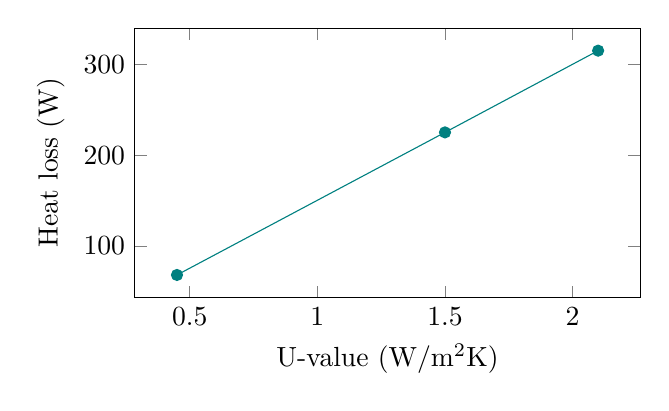
\begin{tikzpicture}
    \begin{axis}[width=8cm, height=5cm, xlabel={U-value (W/m$^2$K)}, ylabel={Heat loss (W)}]
      \addplot[teal, mark=*] coordinates {(0.45,68) (1.5,225) (2.1,315)};
    \end{axis}
  \end{tikzpicture}
  \caption{Heat loss rises in proportion to the U-value.}
  \label{fig:loss}
\end{figure}

\section{Conclusion}
Find this project's source at \url{https://ahmadammar.github.io/teaching/latex/}.

\bibliographystyle{plainnat}
\bibliography{refs}
\end{document}
